\documentclass[10pt,twocolumn,letterpaper]{article}

\usepackage[margin=0.75in,top=0.85in,bottom=0.9in]{geometry}
\usepackage{graphicx}
\usepackage{booktabs}
\usepackage{amsmath}
\usepackage{amssymb}
\usepackage{xcolor}
\usepackage[numbers,sort&compress]{natbib}
\usepackage[colorlinks=true,linkcolor=blue,citecolor=blue,urlcolor=blue]{hyperref}
\usepackage{subcaption}
\usepackage{microtype}
\usepackage{multirow}
\usepackage{array}
\usepackage{enumitem}
\usepackage{float}
\usepackage{caption}
\usepackage{tikz}
\usetikzlibrary{arrows.meta,positioning,shapes.geometric,fit,backgrounds}
\usepackage{setspace}

\graphicspath{{figures/}{../assets/}}

\captionsetup{font=small,labelfont=bf,skip=4pt}
\setlength{\columnsep}{0.22in}

\definecolor{bestcol}{RGB}{0,120,0}
\newcommand{\best}[1]{\textbf{\textcolor{bestcol}{#1}}}
\newcommand{\model}[1]{\textsc{#1}}
\newcommand{\env}[1]{\texttt{#1}}

% ---- Title block -------------------------------------------------------
\title{
  \vspace{-0.5cm}
  \textbf{Image Conditioned Code Generation using RLVR}
  \vspace{-0.3cm}
}

\author{
  Amal Joe R S (24M0797) \quad Job J (25D0364)\\[2pt]
  \small CS 748: Advances in Intelligent and Learning Agents\\
  \small Indian Institute of Technology Bombay\\
  \small Instructor: Prof.\ Shivaram Kalyanakrishnan
}

\date{}

\begin{document}

\maketitle
\thispagestyle{empty}

% ========================================================================
\begin{abstract}
\noindent
We present \model{VisionCoder}, a system for screenshot-to-HTML generation
that trains a vision-language model using reinforcement learning with
verifiable rewards (RLVR). The core problem is that standard supervised
fine-tuning (SFT) does not optimise for rendered visual fidelity: a model
can produce syntactically valid but visually empty HTML and incur no training
loss. We address this by rendering each generated HTML page in a headless
browser and comparing the result to the reference via a composite of eight
sub-rewards covering visual similarity (CLIP, SSIM), spatial layout (position,
color), and semantic structure (text block matching). We fine-tune Qwen 3 VL 4B
in two stages: SFT on 20{,}000 screenshot-HTML pairs with a resolution
curriculum, followed by Group Relative Policy Optimization (GRPO). On the
Design2Code benchmark (484 examples) our SFT+RL model scores
80.5\,/\,91.3\,/\,75.6\,/\,70.2\,/\,89.0 (Block\,/\,Text\,/\,Position\,/\,Color\,/\,CLIP),
outperforming Design2Code-18B on four of five metrics with \textbf{4.5$\times$ fewer
parameters}. We also release \model{VisionCoder-Env}, an OpenEnv environment
that wraps our rendering and reward pipeline as an HTTP API so that any
vision-language model can train on this task.
\end{abstract}

% ========================================================================
\section{Introduction}

Reinforcement learning with verifiable rewards (RLVR) has become a popular
training strategy for large language models.  Systems built on Group Relative
Policy Optimization (GRPO)~\citep{shao2024deepseekmath} and DeepSeek-R1~\citep{deepseek2025r1}
showed that optimising directly against verifiable signals, rather than
token-level cross-entropy, can significantly improve reasoning on math and code,
often matching or beating supervised fine-tuning alone.

RLVR has mostly been applied to text-only tasks.  Whether it works for
image-conditioned generation, where the reward comes from visual comparison
rather than string matching, is much less studied.  We investigate this for
\textbf{screenshot-to-HTML generation}: given a webpage screenshot, produce
HTML and CSS that, when rendered in a browser, visually matches the original.

The task has practical value on two fronts.  Frontend developers spend
considerable time converting UI mockups to code; automating this step speeds
up the prototyping cycle.  Financial regulators also require reports submitted
as structured XHTML, currently produced by expensive PDF-to-HTML conversion
pipelines.  The reward signal is naturally verifiable: render the generated
HTML in a headless browser and compare the screenshot to the reference.
No human annotation is required.

Standard SFT on screenshot-HTML pairs misses this objective.  A model can
generate syntactically valid but visually empty HTML and still see low training
loss, because the loss measures token prediction accuracy, not visual output.
Our approach is to render each candidate in a headless browser via
Playwright~\citep{playwright2023} and score it with a composite visual
similarity metric.  This makes the training signal directly tied to what the
model actually produces on screen.

\paragraph{Contributions.}
\begin{enumerate}[leftmargin=1em,itemsep=1pt,topsep=2pt]
\item \textbf{\model{VisionCoder} model.}  Qwen 3 VL 4B fine-tuned with
      SFT\,+\,GRPO using an 8-component rendering-based reward.  Our SFT+RL
      model outperforms Design2Code-18B~\citep{si2025design2code} on four of
      five benchmark metrics with 4.5$\times$ fewer parameters.
\item \textbf{\model{VisionCoder-Env}.}  A standardized OpenEnv
      environment~\citep{openenv2025} exposing our rendering pipeline and
      reward computation as an HTTP API, so any VLM can train on this task
      without rebuilding the reward infrastructure.  The environment is
      publicly available on the OpenEnv Hub.
\end{enumerate}

% ========================================================================
\section{Related Work}

\paragraph{Screenshot-to-code.}
Beltramelli~\citep{beltramelli2018pix2code} introduced \textit{pix2code}, an
end-to-end CNN\,+\,LSTM system that achieved 77\% accuracy on synthetic GUI
screenshots.  The WebSight dataset~\citep{huggingface2024websight} provides
2\,M synthetic screenshot-HTML pairs and showed that an 8B VLM can be
fine-tuned effectively for this task.  Design2Code~\citep{si2025design2code}
built the first real-world benchmark with 484 webpage examples and an 18B SFT
baseline.  WebCode2M~\citep{webcode2m2024} provides a large-scale real-world
dataset for code generation from webpage designs.  Concurrently, ReLook~\citep{relook2025}
uses a vision-grounded RL loop with an MLLM critic for iterative web coding.
Our work differs in targeting single-pass generation with an automated
composite reward rather than a multi-turn critique loop.

\paragraph{RLVR in LLMs.}
GRPO was introduced in DeepSeekMath~\citep{shao2024deepseekmath} for
mathematical reasoning; it computes group-relative advantages without a
separate critic.  DeepSeek-R1~\citep{deepseek2025r1} showed that pure RL with
verifiable rewards can yield strong reasoning, raising AIME 2024
pass@1 from 15.6\% to 71.0\%.  InstructGPT~\citep{ouyang2022instructgpt}
is the foundational work on using human feedback to align LLMs.

\paragraph{Vision-language models.}
We build on Qwen3-VL~\citep{qwen3vl2025}, which supports dynamic resolution
and a native 256K-token context.  Other relevant VLMs include
LLaVA~\citep{liu2023llava}, Flamingo~\citep{alayrac2022flamingo}, and
InstructBLIP~\citep{dai2023instructblip}.  We use CLIP~\citep{radford2021clip}
(ViT-B/32) for visual reward computation.

% ========================================================================
\section{Problem Formulation}

Given an input image $I \in \mathbb{R}^{H \times W \times 3}$ of a webpage,
the goal is to generate an HTML document $\hat{h}$ such that rendering it in a
browser produces a screenshot $\hat{I}$ that visually matches $I$.
We seek a policy $\pi_\theta$ that maximizes:
\[
  \mathbb{E}_{I \sim \mathcal{D}}\,\mathbb{E}_{\hat{h} \sim \pi_\theta(\cdot|I)}
  \bigl[R(I, \hat{I})\bigr],
\]
where $\hat{I} = \text{Render}(\hat{h})$ and $R$ is the composite reward
function described in Section~\ref{sec:reward}.

\paragraph{Evaluation.}
We evaluate on the Design2Code benchmark~\citep{si2025design2code}: 484 real
webpages, five metrics: \textit{Block} (structural element matching),
\textit{Text} (text content accuracy), \textit{Position} (layout placement),
\textit{Color} (color scheme), and \textit{CLIP} (overall visual similarity).

% ========================================================================
\section{Methodology}

\subsection{Base Model}

We use \textbf{Qwen 3 VL 4B}~\citep{qwen3vl2025} as the base model.
Qwen3-VL supports native dynamic resolution via interleaved-MRoPE, so images
from thumbnail size up to 1920$\times$1080 are processed in a single forward
pass without manual resizing.  At 4B parameters the model is also 4.5$\times$
smaller than the Design2Code-18B baseline, which matters for deployment.

\subsection{SFT with Resolution Curriculum}
\label{sec:sft}

We first fine-tune on \textbf{20{,}000 screenshot-HTML pairs} from
WebSight~\citep{huggingface2024websight} using standard next-token prediction.
Without this step, the HTML action space is so large that early GRPO rollouts
mostly produce invalid or empty pages, giving near-zero rewards and uninformative
advantage estimates.  After SFT, all rollouts for a given prompt produce
parseable HTML from the very first GRPO iteration, so the optimizer can spend
its budget on improving visual quality rather than fixing basic syntax.

Managing vision token count is a practical concern: a 1920$\times$1080 image
produces roughly 9{,}800 tokens with Qwen3-VL, so training entirely at full
resolution is too slow.  We use a \textbf{resolution curriculum}:
\begin{itemize}[leftmargin=1.2em,itemsep=1pt,topsep=2pt]
  \item 60\% of samples at quarter resolution (480$\times$270, $\approx$256 tokens)
  \item 20\% at half resolution (960$\times$540, $\approx$1{,}024 tokens)
  \item 20\% at full resolution (1920$\times$1080, $\approx$9{,}800 tokens)
\end{itemize}
The model first picks up general HTML structure at low cost, then gets exposure
to fine-grained visual detail at full resolution.

\subsection{GRPO Training}

After SFT we run Group Relative Policy Optimization
(GRPO)~\citep{shao2024deepseekmath}.  For each training prompt (a reference
image), the model generates $G = 8$ candidate HTML outputs.  The advantage for
candidate $i$ is:
\[
  A_i = \frac{r_i - \mu_r}{\sigma_r + \epsilon},
\]
where $r_i$ is the reward for candidate $i$ and $\mu_r$, $\sigma_r$ are the
group mean and standard deviation.  The policy gradient is applied over all
tokens in the trajectory weighted by $A_i$.  We use the DR-GRPO loss
(importance sampling disabled), giving a $\sim$38\% speed improvement
over standard GRPO~\citep{vonwerra2022trl}.

For GRPO we also apply a resolution curriculum (50\% at 128$\times$128,
30\% at 256$\times$256, 20\% at 512$\times$512) to keep GPU memory under
control when running 8 rollouts per prompt.  Training runs for \textbf{500 steps}
on \textbf{4$\times$ NVIDIA A100 80\,GB GPUs}, taking roughly 2 days.

\begin{figure*}[t]
  \centering
  \resizebox{\textwidth}{!}{%
  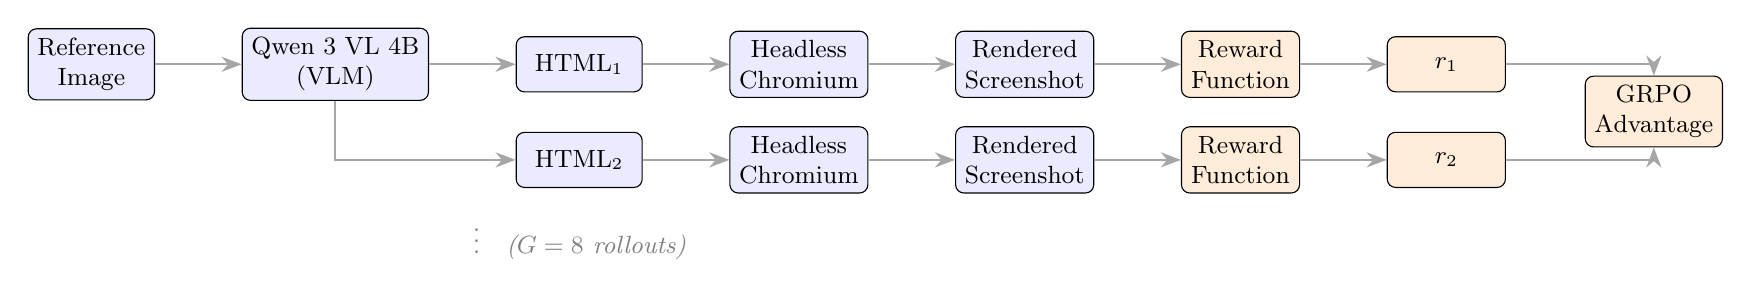
\begin{tikzpicture}[
    node distance=1.1cm,
    box/.style={draw, rounded corners=3pt, fill=blue!8,
                minimum height=0.7cm, minimum width=1.6cm,
                font=\small, align=center},
    reward/.style={draw, rounded corners=3pt, fill=orange!15,
                   minimum height=0.7cm, minimum width=1.5cm,
                   font=\small, align=center},
    arrow/.style={-{Stealth[scale=1.1]}, thick, gray!70},
    grp/.style={draw=gray!40, dashed, rounded corners=5pt,
                inner sep=5pt, fill=gray!5}
  ]

  \node[box] (img) {Reference\\Image};
  \node[box, right=of img] (vlm) {Qwen 3 VL 4B\\(VLM)};
  \node[box, right=of vlm] (html1) {HTML$_1$};
  \node[box, right=of html1] (browser) {Headless\\Chromium};
  \node[box, right=of browser] (rend1) {Rendered\\Screenshot};
  \node[reward, right=of rend1] (rfn) {Reward\\Function};
  \node[reward, right=of rfn] (r1) {$r_1$};

  \node[box, below=0.5cm of html1] (html2) {HTML$_2$};
  \node[box, right=of html2] (browser2) {Headless\\Chromium};
  \node[box, right=of browser2] (rend2) {Rendered\\Screenshot};
  \node[reward, right=of rend2] (rfn2) {Reward\\Function};
  \node[reward, right=of rfn2] (r2) {$r_2$};

  \node[below=0.18cm of html2, font=\small\itshape, text=gray] (dots) {$\vdots$\quad ($G=8$ rollouts)};

  \draw[arrow] (img) -- (vlm);
  \draw[arrow] (vlm) -- (html1);
  \draw[arrow] (html1) -- (browser);
  \draw[arrow] (browser) -- (rend1);
  \draw[arrow] (rend1) -- (rfn);
  \draw[arrow] (rfn) -- (r1);

  \draw[arrow] (vlm.south) |- (html2.west);
  \draw[arrow] (html2) -- (browser2);
  \draw[arrow] (browser2) -- (rend2);
  \draw[arrow] (rend2) -- (rfn2);
  \draw[arrow] (rfn2) -- (r2);

  % GRPO advantage box
  \node[reward, right=1.0cm of r1, yshift=-0.6cm] (grpo) {GRPO\\Advantage};
  \draw[arrow] (r1.east) -| (grpo.north);
  \draw[arrow] (r2.east) -| (grpo.south);

  \end{tikzpicture}}%
  \caption{RLVR training loop. For each reference image the VLM generates
    $G=8$ HTML candidates; each is rendered in a headless browser and
    scored by the composite reward function. GRPO computes group-relative
    advantages to update the policy.}
  \label{fig:arch}
\end{figure*}

\subsection{Composite Reward Function}
\label{sec:reward}

The reward function combines eight sub-rewards, each targeting a different
quality dimension (Figure~\ref{fig:reward_weights}):

\vspace{2pt}
\noindent\textbf{Format} ($w\!=\!0.5$). Checks for a Markdown HTML fence
(\texttt{```html~...~```}) and a valid \texttt{<!DOCTYPE html>} declaration.

\noindent\textbf{Validity} ($w\!=\!0.5$). Checks for \texttt{<html>},
\texttt{<head>}, \texttt{<body>} (weighted 0.5) and tag diversity
($\min(\text{unique tags}/8, 1.0)$, weighted 0.5).

\noindent\textbf{Structural} ($w\!=\!0.5$). Tag sequence similarity via
longest-common-subsequence (LCS) ratio, plus CSS class Jaccard similarity
between prediction and reference.

\noindent\textbf{Text Block} ($w\!=\!3.4$, highest weight). Extracts visible
text DOM nodes from both renders using Playwright, applies the Hungarian
algorithm for optimal IoU-based block matching, then measures character-level
text similarity per matched pair.  This sub-reward carries the most weight
because text content and its spatial placement are what users notice first.

\noindent\textbf{Position} ($w\!=\!1.0$). For each matched block pair,
computes $1.0 - \|\mathbf{c}_\text{pred} - \mathbf{c}_\text{ref}\|_2 / d_\text{diag}$,
where $d_\text{diag}$ is the viewport diagonal.

\noindent\textbf{Color} ($w\!=\!2.5$). Downsamples to 128$\times$128,
converts to CIELAB, and computes mean CIEDE2000~\citep{sharma2005ciede2000}
distance $\Delta E_{00}$ over non-white reference pixels:
$r_\text{col} = 1 - \min(\overline{\Delta E_{00}}/50, 1)$.
Restricting to non-white pixels avoids penalising for shared background color.

\noindent\textbf{CLIP} ($w\!=\!1.3$). Cosine similarity of CLIP
ViT-B/32~\citep{radford2021clip} embeddings, re-normalised via
$\max(0, (s - 0.65)/0.35)$ to push blank pages toward zero while preserving
sensitivity in the high-quality range.

\noindent\textbf{SSIM} ($w\!=\!1.3$). Structural Similarity
Index~\citep{wang2004ssim} at 320$\times$240 RGB, which picks up
luminance and contrast differences that CLIP misses in the 0.7--0.97 range.

\vspace{4pt}
The composite reward is:
\begin{align}
  r_\text{total} &= \frac{1}{11.0}\bigl(
    0.5\,r_\text{fmt} + 0.5\,r_\text{val} + 0.5\,r_\text{str}\nonumber\\
  &\quad + 3.4\,r_\text{txt} + 1.0\,r_\text{pos} + 2.5\,r_\text{col}\nonumber\\
  &\quad + 1.3\,r_\text{clip} + 1.3\,r_\text{ssim}\bigr)
  \label{eq:reward}
\end{align}

\noindent A \textbf{blank-page guard} sets $r_\text{total}\!=\!0$ if the
predicted render has fewer than 0.5\% non-white pixels while the reference has
content, preventing the model from gaming the reward with an empty page.

\paragraph{Weight selection.}
Weights were chosen via grid search over candidate combinations, scoring each
by Spearman rank correlation with human quality judgements across 15 reference
webpages rated at 7 quality levels from blank to pixel-perfect.  The final
weights achieve $\rho\!=\!0.955$ (Figure~\ref{fig:reward_validation}).

% ========================================================================
\section{VisionCoder Environment}
\label{sec:env}

\begin{figure*}[t]
  \centering
  \resizebox{0.80\textwidth}{!}{%
  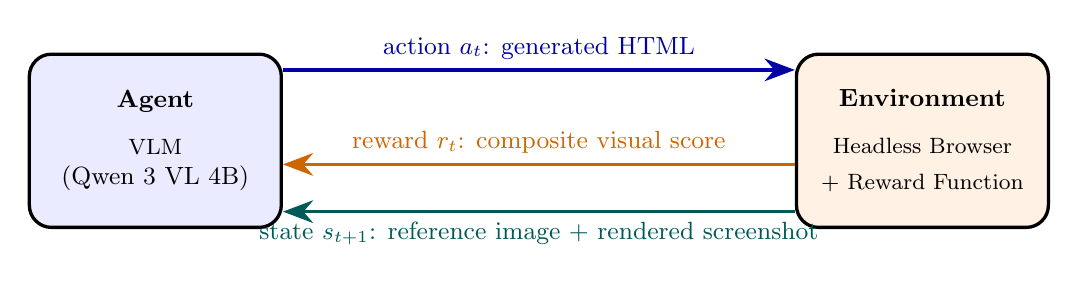
\begin{tikzpicture}[
    mainbox/.style={draw, very thick, rounded corners=8pt,
                    minimum width=3.2cm, minimum height=2.2cm,
                    align=center, font=\small},
    arrow/.style={-{Stealth[scale=1.3]}, very thick},
  ]

  \node[mainbox, fill=blue!8] (agent)
      {\textbf{Agent}\\[6pt]\footnotesize VLM\\(Qwen 3 VL 4B)};

  \node[mainbox, fill=orange!10, right=6.5cm of agent] (env)
      {\textbf{Environment}\\[6pt]\footnotesize Headless Browser\\[2pt]\footnotesize + Reward Function};

  % Action: agent → env
  \draw[arrow, blue!65!black]
    ([yshift=9mm]agent.east) --
    node[above, font=\small, text=blue!65!black]
        {action $a_t$: generated HTML}
    ([yshift=9mm]env.west);

  % Reward: env → agent
  \draw[arrow, orange!80!black]
    ([yshift=-3mm]env.west) --
    node[above, font=\small, text=orange!80!black]
        {reward $r_t$: composite visual score}
    ([yshift=-3mm]agent.east);

  % State: env → agent
  \draw[arrow, teal!70!black]
    ([yshift=-9mm]env.west) --
    node[below, font=\small, text=teal!70!black]
        {state $s_{t+1}$: reference image $+$ rendered screenshot}
    ([yshift=-9mm]agent.east);

  \end{tikzpicture}}%
  \caption{\model{VisionCoder-Env} agent-environment loop. The agent (VLM)
    generates HTML ($a_t$); the environment renders it in a headless browser,
    computes the eight-component composite reward $r_t$, and returns the
    updated state $s_{t+1}$ (reference image and new rendered screenshot).
    This loop enables iterative refinement across multiple turns.}
  \label{fig:env}
\end{figure*}

Alongside the trained model we release \textbf{\model{VisionCoder-Env}}, an
environment built on the OpenEnv framework~\citep{openenv2025}, an open-source
platform for agentic RL environments launched by Meta PyTorch and HuggingFace.
The environment exposes our headless Chromium renderer and eight-component
reward function through a simple HTTP API (Figure~\ref{fig:env} shows
the agent-environment loop):

\begin{itemize}[leftmargin=1.2em,itemsep=1pt,topsep=2pt]
  \item \env{POST /reset?difficulty=\{easy|medium|hard\}} $\to$
        \env{\{session\_id, screenshot\_b64\}}
  \item \env{POST /step \{html, session\_id\}} $\to$
        \env{\{reward, render, done\}}
  \item \env{POST /render \{html\}} $\to$ \env{\{image\_b64\}}
\end{itemize}

Three difficulty levels are available: \textit{easy} (login forms, single-column
layouts), \textit{medium} (multi-section pages with navigation), and
\textit{hard} (dashboards with nested flex/grid structures).  The API lets any
VLM of any size or architecture train on this task; the rendering and reward
calculation all happen server-side.

\paragraph{OpenEnv hackathon.}
\model{VisionCoder-Env} was submitted to Meta's OpenEnv hackathon and
shortlisted to the \textbf{top 100 out of 2{,}000 participants}.

% ========================================================================
\section{Experiments}

\subsection{Experimental Setup}

\paragraph{Hardware.} All runs use 4$\times$ NVIDIA A100 80\,GB GPUs with
Accelerate~\citep{gugger2022accelerate} for distributed training.

\paragraph{Datasets.}
SFT uses 20{,}000 samples from WebSight~\citep{huggingface2024websight}.
GRPO uses a disjoint set of 2{,}000 WebSight samples.  We evaluate on the
full Design2Code benchmark~\citep{si2025design2code} (484 held-out webpages).

\paragraph{Inference.}
We serve the model with vLLM at 32 concurrent requests and run predictions
for the full benchmark in a single pass.  The HTML is extracted from the
model's Markdown fenced block before evaluation.

\subsection{Main Results}

Table~\ref{tab:results} shows results on Design2Code.  Our SFT+RL model gets
the best scores among all sub-18B models on Block, Position, Color, and CLIP.
It beats the 18B Design2Code SFT model on four metrics (Block: $+2.0$,
Position: $+1.3$, Color: $+3.2$, CLIP: $+3.2$) while using 4.5$\times$
fewer parameters.  The only metric where the larger model wins is Text ($+5.1$),
which is likely because a bigger model can memorise finer character-level
details.

Even the \textbf{RL-only} model (500 GRPO steps from the base, no SFT)
scores 79.5/88.4/70.6/69.8/85.9, which is already competitive with
Design2Code-18B on most metrics.  This shows that the rendering-based reward
alone is informative enough to pull a 4B base model from near-zero to a
useful regime.

\begin{table}[t]
\centering
\caption{Design2Code benchmark results (484 examples). All scores are
percentages. Best non-GPT-4o scores are \best{highlighted}.}
\label{tab:results}
\renewcommand{\arraystretch}{1.1}
\setlength{\tabcolsep}{3pt}
\footnotesize
\begin{tabular}{lrrrrr}
\toprule
\textbf{Model} & \textbf{Blk} & \textbf{Txt} & \textbf{Pos} & \textbf{Col} & \textbf{CLIP} \\
\midrule
GPT-4o             & 93.0 & 98.2 & 85.5 & 84.1 & 90.4 \\
\midrule
Design2Code-18B    & 78.5 & \best{96.4} & 74.3 & 67.0 & 85.8 \\
LLaVA 1.6-7B       & 50.4 & 87.9 & 69.1 & 63.4 & 84.6 \\
DeepSeek-VL-7B     & 39.7 & 77.0 & 64.6 & 63.8 & 84.5 \\
Qwen 3 VL 4B (Base)& 10.1 & 10.8 &  8.8 &  9.1 & 77.2 \\
\midrule
\model{VisionCoder} (RL only)   & 79.5 & 88.4 & 70.6 & 69.8 & 85.9 \\
\model{VisionCoder} (SFT+RL)    & \best{80.5} & 91.3 & \best{75.6} & \best{70.2} & \best{89.0} \\
\bottomrule
\end{tabular}
\end{table}

\subsection{Ablation: RL-only vs.\ SFT+RL}

Adding SFT before GRPO improves all five metrics, with the biggest gains in
Text ($+2.9$) and CLIP ($+3.1$).  Without SFT, many early GRPO rollouts
produce broken or empty HTML; the resulting near-zero rewards give all
candidates similar advantages, making the gradient step nearly uninformative.
With SFT, even the worst rollout in a group produces parseable HTML with
some structural match to the reference, so the relative ordering within the
group is meaningful from the start.

\subsection{Training Dynamics}

Figure~\ref{fig:training} tracks reward components and completion lengths
over 500 GRPO steps.  In the first 100 steps, format and validity rewards
jump to near-perfect; the model quickly learns the output contract (HTML fence,
DOCTYPE, required tags) and the gradient signal shifts entirely to visual
metrics.  After step 100, CLIP and SSIM rise steadily while the total reward
climbs from roughly 2.4 to 5.0.  Completion length drops sharply from around
1{,}000 tokens to around 460: the model learns to write compact HTML
rather than filling the context with redundant tags and inline comments.

\begin{figure}[t]
  \centering
  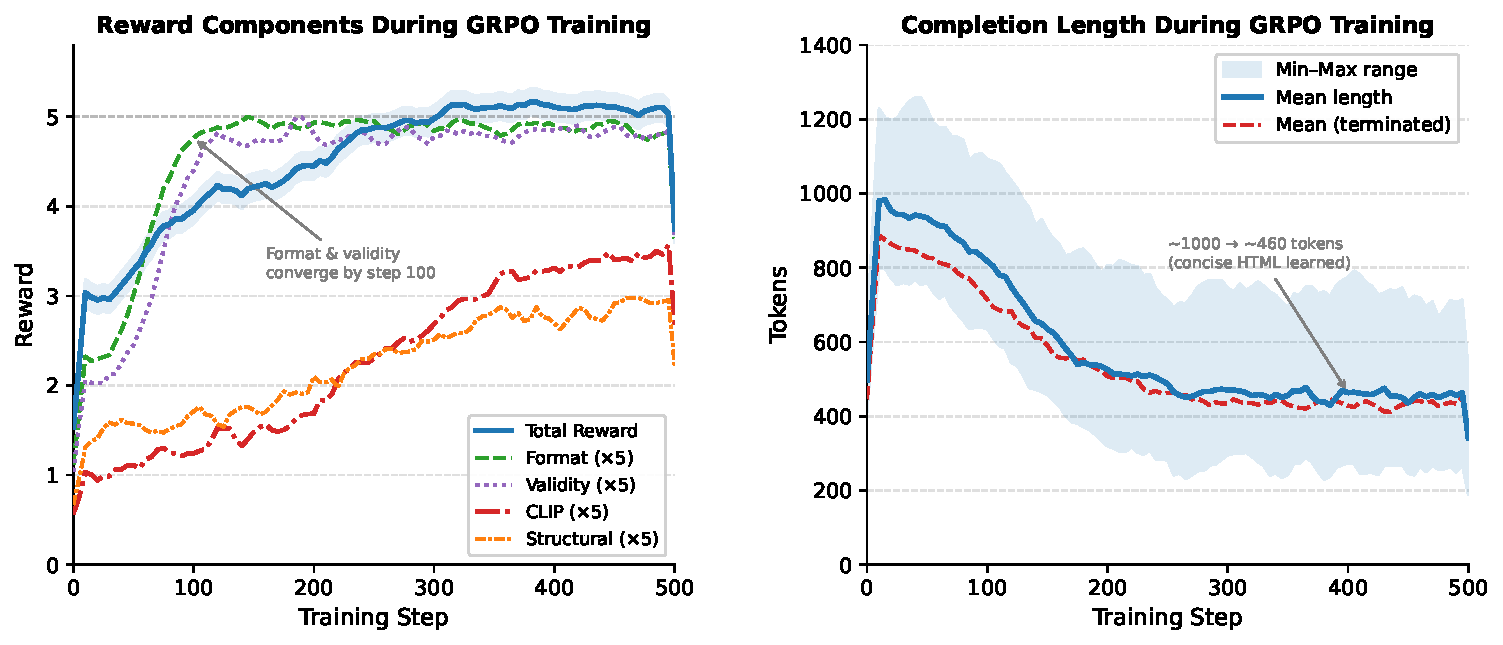
\includegraphics[width=\columnwidth]{training_curves.pdf}
  \caption{Training dynamics over 500 GRPO steps. \textit{Left:} Total reward
    and scaled component rewards. Format and validity stabilise by step~100;
    CLIP and SSIM rise steadily after that. \textit{Right:} Completion length
    drops from $\approx$1{,}000 to $\approx$460 tokens as the model learns
    to write concise HTML.}
  \label{fig:training}
\end{figure}

\begin{figure}[t]
  \centering
  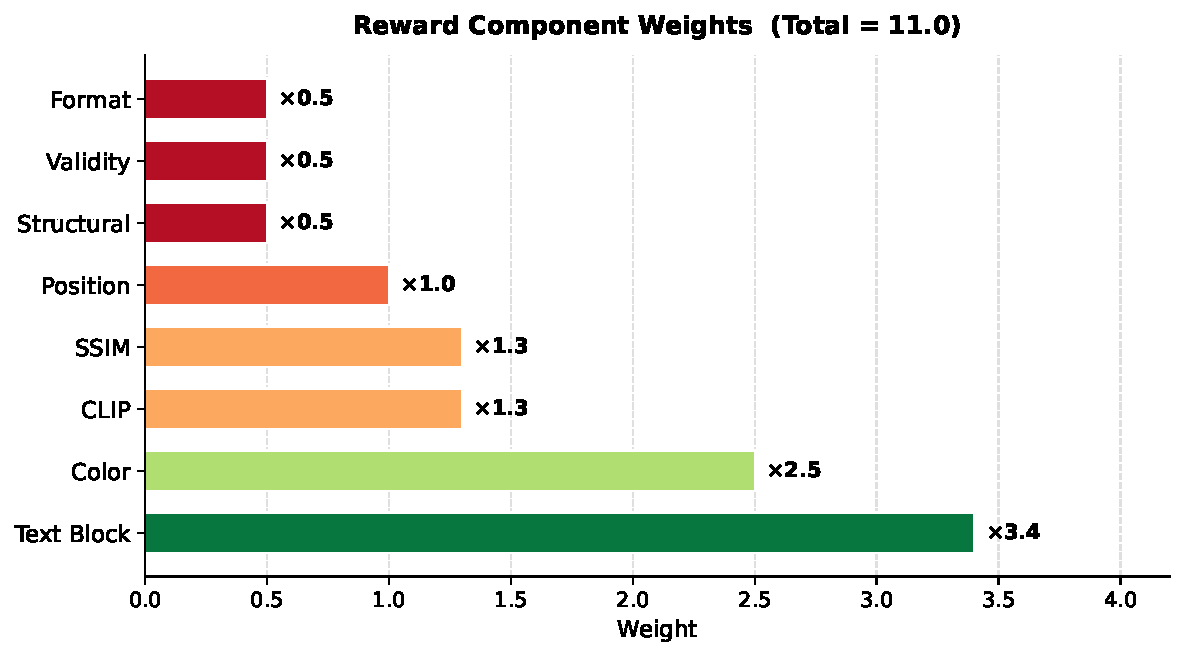
\includegraphics[width=\columnwidth]{reward_weights.pdf}
  \caption{Reward component weights in Eq.~\ref{eq:reward}. Text-Block has the
    highest weight (3.4) because text content and placement are the most
    immediately perceptible quality dimensions.}
  \label{fig:reward_weights}
\end{figure}

\begin{figure}[t]
  \centering
  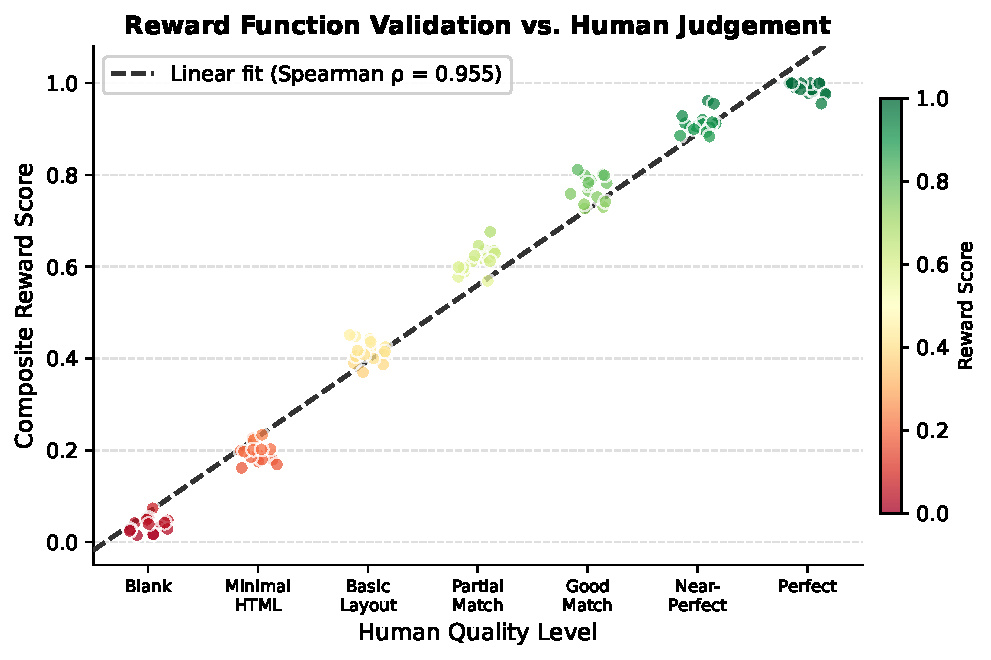
\includegraphics[width=\columnwidth]{reward_validation.pdf}
  \caption{Composite reward score vs.\ human quality rank across 7 quality
    levels and 15 reference webpages (Spearman $\rho\!=\!0.955$).}
  \label{fig:reward_validation}
\end{figure}

\subsection{Qualitative Results}

Figure~\ref{fig:qualitative} shows reference-prediction pairs from
VisionCoder-Env at three difficulty levels.  Easy examples (simple
single-column pages) come out very close to the reference
(Block\,91.0, CLIP\,98.4).  Medium examples (multi-section pages) reproduce
content and color well with only small positional offsets
(Block\,90.0, CLIP\,96.4).  Hard examples (complex multi-column dashboards)
are only partially reproduced (Block\,75.3, CLIP\,58.0); deeply nested
CSS grid and flex structures are where the model still struggles most.

\begin{figure}[t]
  \centering
  \begin{subfigure}[b]{0.49\columnwidth}
    
\includegraphics[width=\linewidth]{../assets/qual_openenv/after/easy_0_ref.png}
    \caption*{Reference (easy)}
  \end{subfigure}
  \hfill
  \begin{subfigure}[b]{0.49\columnwidth}
    
\includegraphics[width=\linewidth]{../assets/qual_openenv/after/easy_0_pred.png}
    \caption*{Prediction (easy)}
  \end{subfigure}

  \vspace{3pt}
  \begin{subfigure}[b]{0.49\columnwidth}
    
\includegraphics[width=\linewidth]{../assets/qual_openenv/after/medium_0_ref.png}
    \caption*{Reference (medium)}
  \end{subfigure}
  \hfill
  \begin{subfigure}[b]{0.49\columnwidth}
    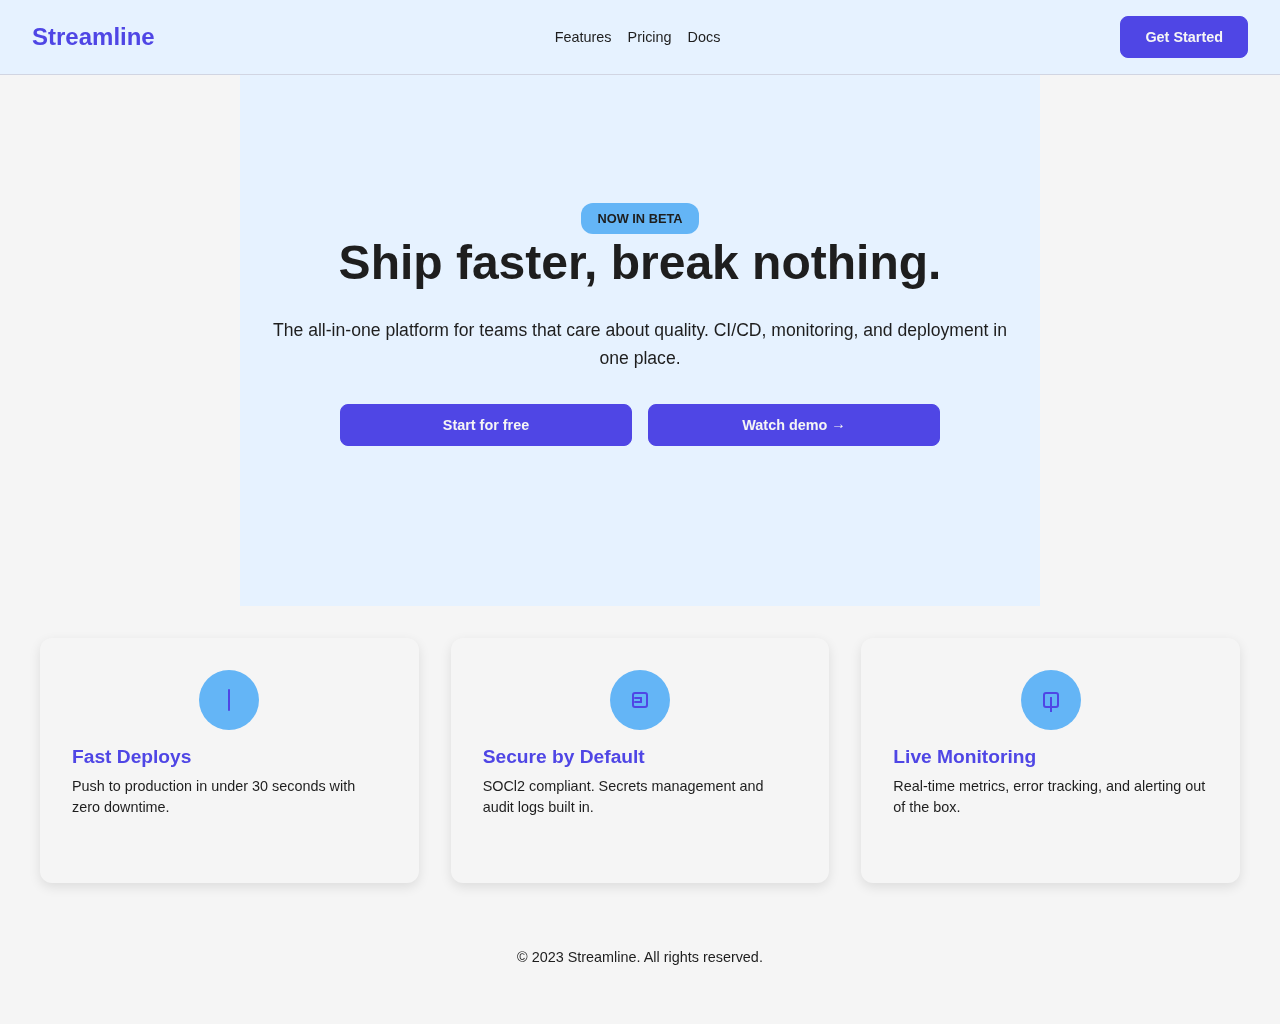
\includegraphics[width=\linewidth]{../assets/qual_openenv/after/medium_0_pred.png}
    \caption*{Prediction (medium)}
  \end{subfigure}

  \vspace{3pt}
  \begin{subfigure}[b]{0.49\columnwidth}
    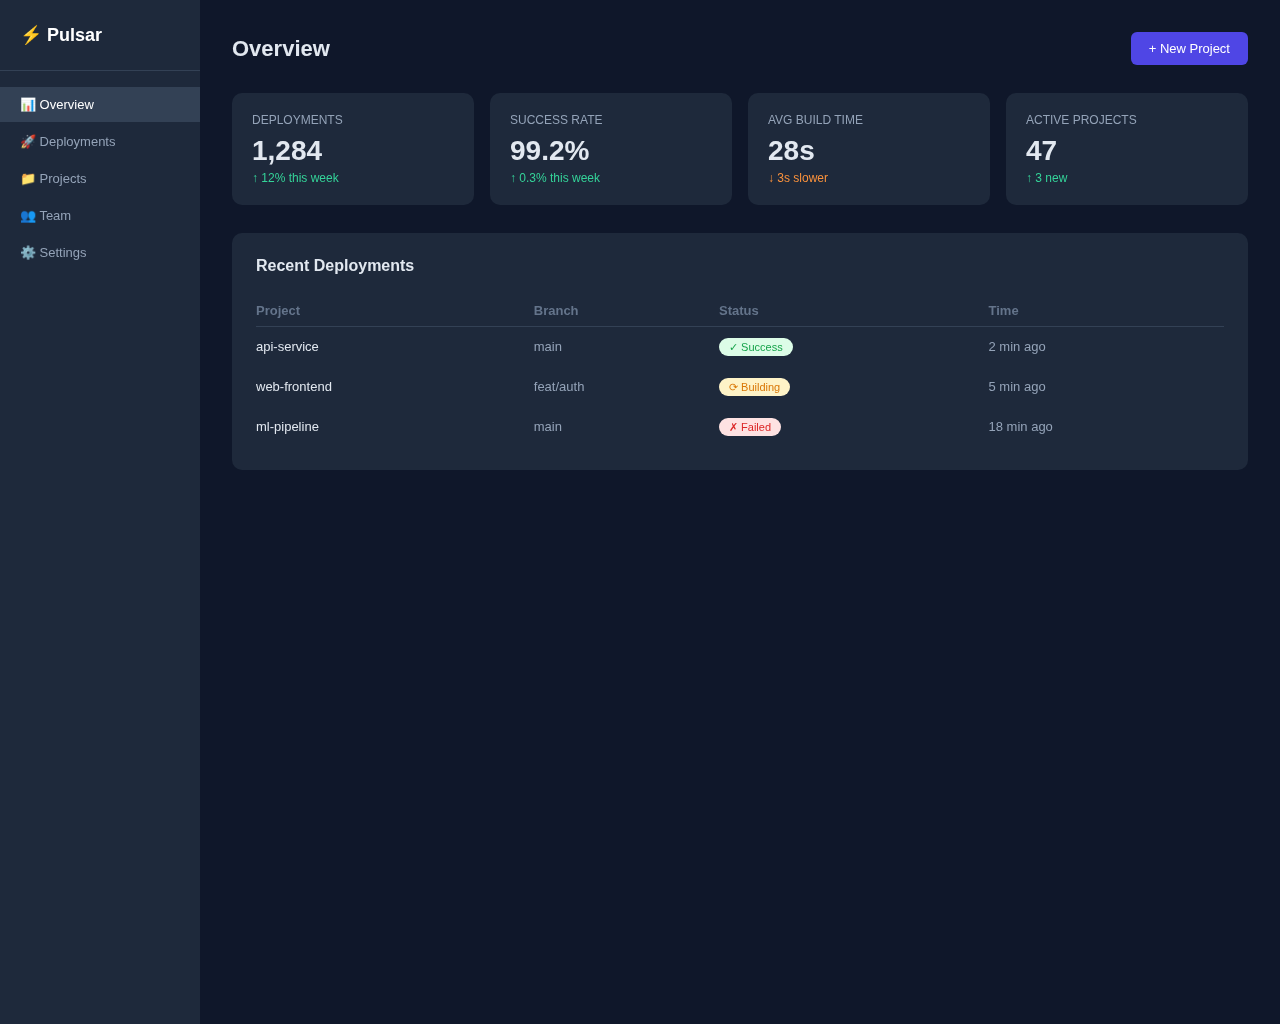
\includegraphics[width=\linewidth]{../assets/qual_openenv/after/hard_0_ref.png}
    \caption*{Reference (hard)}
  \end{subfigure}
  \hfill
  \begin{subfigure}[b]{0.49\columnwidth}
    
\includegraphics[width=\linewidth]{../assets/qual_openenv/after/hard_0_pred.png}
    \caption*{Prediction (hard)}
  \end{subfigure}

  \caption{Reference-prediction pairs at three difficulty levels. Easy and
    medium pages are reproduced with high fidelity. Hard examples with deeply
    nested grid/flex layouts remain the main failure mode.}
  \label{fig:qualitative}
\end{figure}

\begin{figure*}[t]
  \centering
  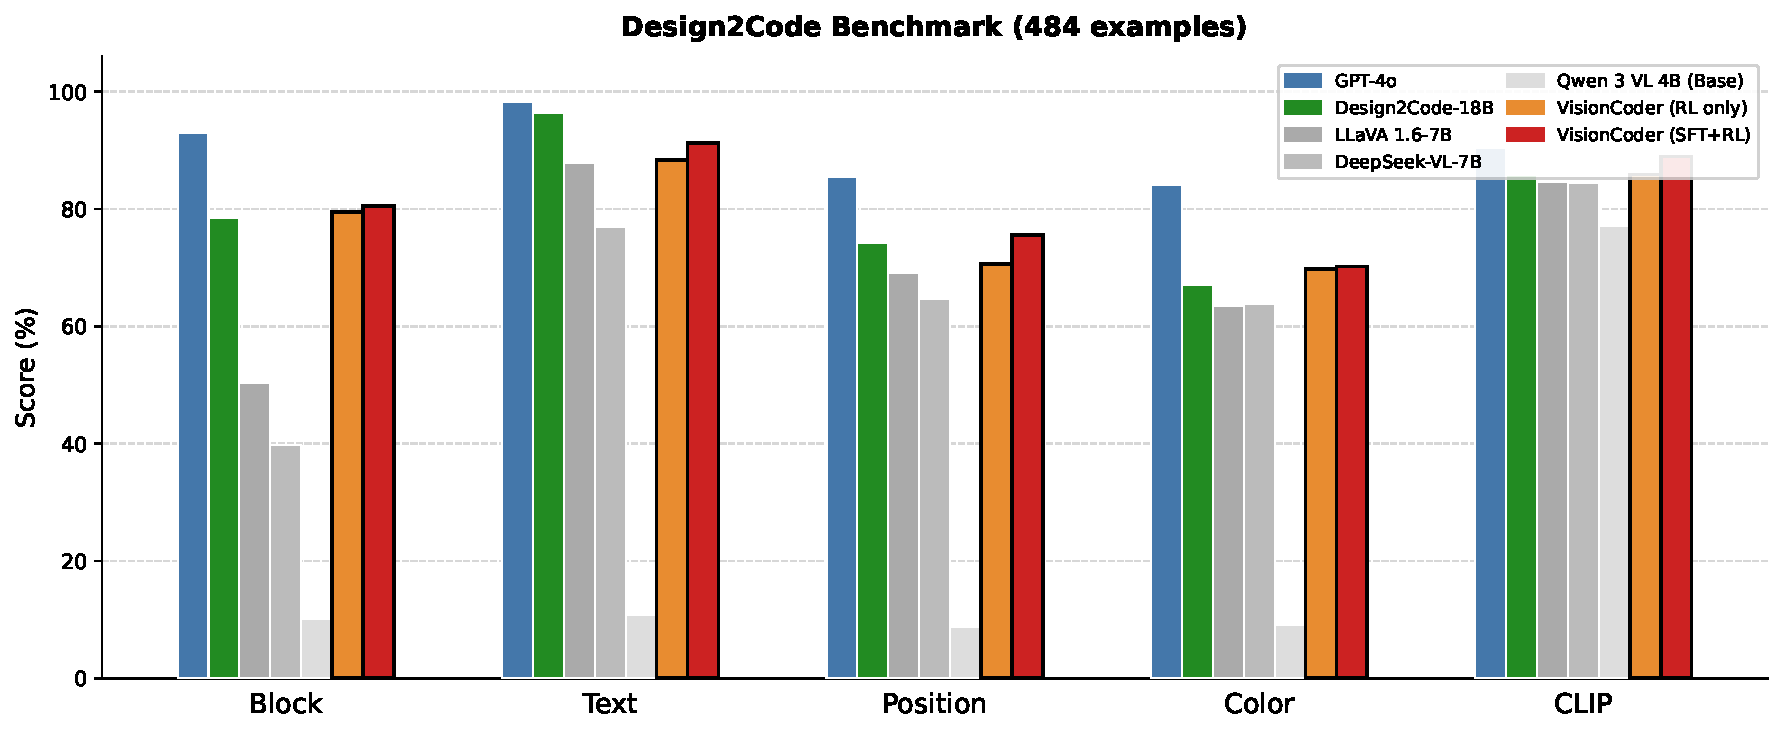
\includegraphics[width=0.85\textwidth]{design2code_results.pdf}
  \caption{Design2Code benchmark comparison. \model{VisionCoder} (SFT+RL,
    4B params) outperforms Design2Code-18B on Block, Position, Color, and
    CLIP with 4.5$\times$ fewer parameters. Only Text favours the larger model.}
  \label{fig:results}
\end{figure*}


% ========================================================================
\section{Conclusion}

We showed that RLVR with a rendering-based reward is a viable training
approach for screenshot-to-HTML generation.  A few things stood out.  RL alone,
without any SFT, already brings a 4B base model up to the level of the 18B
Design2Code SFT baseline, which is more than we initially expected from 500
training steps.  Adding SFT first makes a meaningful further difference across
all metrics, mainly by giving the model a stable starting point so early GRPO
gradients are useful rather than noisy.  Getting the reward function right
matters a lot: a single metric like CLIP is not enough, and the eight-component
composite (validated at Spearman $\rho\!=\!0.955$) gives a much cleaner signal.
Finally, wrapping the reward pipeline in \model{VisionCoder-Env} means any
future model can plug in and train on this task without reimplementing the
rendering stack.

The main remaining gap is on complex multi-column layouts, where the model
sometimes gets the content right but places elements in the wrong region.
A natural next step is iterative refinement: let the model see its rendered
output and revise it over a few turns, along the lines of
ReLook~\citep{relook2025}.  Extending the pipeline to PDF-to-XHTML conversion
for financial filings is another direction with direct practical value.

\paragraph{Acknowledgements.}
We thank Prof.\ Shivaram Kalyanakrishnan for guidance throughout this project.
Compute was provided by IIT Bombay HPC facilities.

\bibliographystyle{abbrvnat}
\bibliography{refs}

\end{document}
